\documentclass[a4paper,11pt]{book}
%\documentclass[a4paper,twoside,11pt,titlepage]{book}
\usepackage{listings}
\usepackage[utf8]{inputenc}
\usepackage[spanish]{babel}

% \usepackage[style=list, number=none]{glossary} %
%\usepackage{titlesec}
%\usepackage{pailatino}

\decimalpoint
\usepackage{dcolumn}
\newcolumntype{.}{D{.}{\esperiod}{-1}}
\makeatletter
\addto\shorthandsspanish{\let\esperiod\es@period@code}
\makeatother


%\usepackage[chapter]{algorithm}
\RequirePackage{verbatim}
%\RequirePackage[Glenn]{fncychap}
\usepackage{fancyhdr}
\usepackage{graphicx}
\usepackage{afterpage}

\usepackage{longtable}

\usepackage[pdfborder={000}]{hyperref} %referencia

\usepackage{natbib} % Paquete para la gestión de la bibliografía

% ********************************************************************
% Re-usable information
% ********************************************************************
\newcommand{\myTitle}{Título del proyecto\xspace}
\newcommand{\myDegree}{Grado en ...\xspace}
\newcommand{\myName}{Nombre Apllido1 Apellido2 (alumno)\xspace}
\newcommand{\myProf}{Nombre Apllido1 Apellido2 (tutor1)\xspace}
\newcommand{\myOtherProf}{Nombre Apllido1 Apellido2 (tutor2)\xspace}
%\newcommand{\mySupervisor}{Put name here\xspace}
\newcommand{\myFaculty}{Escuela Técnica Superior de Ingenierías Informática y de
Telecomunicación\xspace}
\newcommand{\myFacultyShort}{E.T.S. de Ingenierías Informática y de
Telecomunicación\xspace}
\newcommand{\myDepartment}{Departamento de ...\xspace}
\newcommand{\myUni}{\protect{Universidad de Granada}\xspace}
\newcommand{\myLocation}{Granada\xspace}
\newcommand{\myTime}{\today\xspace}
\newcommand{\myVersion}{Version 0.1\xspace}


\hypersetup{
pdfauthor = {\myName (email (en) ugr (punto) es)},
pdftitle = {\myTitle},
pdfsubject = {},
pdfkeywords = {palabra_clave1, palabra_clave2, palabra_clave3, ...},
pdfcreator = {LaTeX con el paquete ....},
pdfproducer = {pdflatex}
}

%\hyphenation{}


%\usepackage{doxygen/doxygen}
%\usepackage{pdfpages}
\usepackage{url}
\usepackage{colortbl,longtable}
\usepackage[stable]{footmisc}
%\usepackage{index}

%\makeindex
%\usepackage[style=long, cols=2,border=plain,toc=true,number=none]{glossary}
% \makeglossary

% Definición de comandos que me son tiles:
%\renewcommand{\indexname}{Índice alfabético}
%\renewcommand{\glossaryname}{Glosario}

\pagestyle{fancy}
\fancyhf{}
\fancyhead[LO]{\leftmark}
\fancyhead[RE]{\rightmark}
\fancyhead[RO,LE]{\textbf{\thepage}}
\renewcommand{\chaptermark}[1]{\markboth{\textbf{#1}}{}}
\renewcommand{\sectionmark}[1]{\markright{\textbf{\thesection. #1}}}

\setlength{\headheight}{1.5\headheight}

\newcommand{\HRule}{\rule{\linewidth}{0.5mm}}
%Definimos los tipos teorema, ejemplo y definición podremos usar estos tipos
%simplemente poniendo \begin{teorema} \end{teorema} ...
\newtheorem{teorema}{Teorema}[chapter]
\newtheorem{ejemplo}{Ejemplo}[chapter]
\newtheorem{definicion}{Definición}[chapter]

\definecolor{gray97}{gray}{.97}
\definecolor{gray75}{gray}{.75}
\definecolor{gray45}{gray}{.45}
\definecolor{gray30}{gray}{.94}

\lstset{ frame=Ltb,
     framerule=0.5pt,
     aboveskip=0.5cm,
     framextopmargin=3pt,
     framexbottommargin=3pt,
     framexleftmargin=0.1cm,
     framesep=0pt,
     rulesep=.4pt,
     backgroundcolor=\color{gray97},
     rulesepcolor=\color{black},
     %
     stringstyle=\ttfamily,
     showstringspaces = false,
     basicstyle=\scriptsize\ttfamily,
     commentstyle=\color{gray45},
     keywordstyle=\bfseries,
     %
     numbers=left,
     numbersep=6pt,
     numberstyle=\tiny,
     numberfirstline = false,
     breaklines=true,
   }
 
% minimizar fragmentado de listados
\lstnewenvironment{listing}[1][]
   {\lstset{#1}\pagebreak[0]}{\pagebreak[0]}

\lstdefinestyle{CodigoC}
   {
	basicstyle=\scriptsize,
	frame=single,
	language=C,
	numbers=left
   }
\lstdefinestyle{CodigoC++}
   {
	basicstyle=\small,
	frame=single,
	backgroundcolor=\color{gray30},
	language=C++,
	numbers=left
   }

 
\lstdefinestyle{Consola}
   {basicstyle=\scriptsize\bf\ttfamily,
    backgroundcolor=\color{gray30},
    frame=single,
    numbers=none
   }


\newcommand{\bigrule}{\titlerule[0.5mm]}


%Para conseguir que en las páginas en blanco no ponga cabecerass
\makeatletter
\def\clearpage{%
  \ifvmode
    \ifnum \@dbltopnum =\m@ne
      \ifdim \pagetotal <\topskip
        \hbox{}
      \fi
    \fi
  \fi
  \newpage
  \thispagestyle{empty}
  \write\m@ne{}
  \vbox{}
  \penalty -\@Mi
}
\makeatother

\usepackage{pdfpages}
\begin{document}
\begin{titlepage}
 
 
\newlength{\centeroffset}
\setlength{\centeroffset}{-0.5\oddsidemargin}
\addtolength{\centeroffset}{0.5\evensidemargin}
\thispagestyle{empty}

\noindent\hspace*{\centeroffset}\begin{minipage}{\textwidth}

\centering

\includegraphics[width=0.9\textwidth]{imagenes/logo_ugr.jpg}\\[1.4cm]

\textsc{ \Large TRABAJO FIN DE GRADO\\[0.2cm]}
\textsc{ INGENIERÍA EN ...}\\[1cm]
% Upper part of the page
% 
% Title
{\Huge\bfseries Titulo del Proyecto\\
}
\noindent\rule[-1ex]{\textwidth}{3pt}\\[3.5ex]
{\large\bfseries Subtitulo del Proyecto}
\end{minipage}

\vspace{2.5cm}
\noindent\hspace*{\centeroffset}\begin{minipage}{\textwidth}
\centering

\textbf{Autor}\\ {Nombre Apellido1 Apellido2 (alumno)}\\[2.5ex]
\textbf{Directores}\\
{Nombre Apellido1 Apellido2 (tutor1)\\
Nombre Apellido1 Apellido2 (tutor2)}\\[2cm]

\includegraphics[width=0.3\textwidth]{imagenes/etsiit_logo.png}\\[0.1cm]
\textsc{Escuela Técnica Superior de Ingenierías Informática y de Telecomunicación}\\
\textsc{---}\\
Granada, mes de 201
\end{minipage}
%\addtolength{\textwidth}{\centeroffset}
%\vspace{\stretch{2}}
\end{titlepage}



\chapter*{}
%\thispagestyle{empty}
%\cleardoublepage

%\thispagestyle{empty}

\begin{titlepage}
 
 
\setlength{\centeroffset}{-0.5\oddsidemargin}
\addtolength{\centeroffset}{0.5\evensidemargin}
\thispagestyle{empty}

\noindent\hspace*{\centeroffset}\begin{minipage}{\textwidth}

\centering
%
\includegraphics[width=0.9\textwidth]{imagenes/logo_ugr.jpg}\\[1.4cm]

%\textsc{ \Large PROYECTO FIN DE CARRERA\\[0.2cm]}
%\textsc{ INGENIERÍA EN INFORMÁTICA}\\[1cm]
% Upper part of the page
% 

 \vspace{3.3cm}

%si el proyecto tiene logo poner aquí

\includegraphics{imagenes/logo.png} 
 \vspace{0.5cm}

% Title

{\Huge\bfseries Título del proyecto\\
}
\noindent\rule[-1ex]{\textwidth}{3pt}\\[3.5ex]
{\large\bfseries Subtítulo del proyecto.\\[4cm]}
\end{minipage}

\vspace{2.5cm}
\noindent\hspace*{\centeroffset}\begin{minipage}{\textwidth}
\centering

\textbf{Autor}\\ {Nombre Apellido1 Apellido2 (alumno)}\\[2.5ex]
\textbf{Directores}\\
{Nombre Apellido1 Apellido2 (tutor1)\\
Nombre Apellido1 Apellido2 (tutor2)}\\[2cm]
%
\includegraphics[width=0.15\textwidth]{imagenes/tstc.png}\\[0.1cm]
%\textsc{Departamento de Teoría de la Señal, Telemática y Comunicaciones}\\
%\textsc{---}\\
%Granada, mes de 201
\end{minipage}
%\addtolength{\textwidth}{\centeroffset}
\vspace{\stretch{2}}

 
\end{titlepage}






\cleardoublepage
\thispagestyle{empty}

\begin{center}
{\large\bfseries Título del Proyecto: Subtítulo del proyecto}\\
\end{center}
\begin{center}
Nombre Apellido1 Apellido2 (alumno)\\
\end{center}

%\vspace{0.7cm}
\noindent{\textbf{Palabras clave}: palabra\_clave1, palabra\_clave2, palabra\_clave3, ......}\\

\vspace{0.7cm}
\noindent{\textbf{Resumen}}\\

Poner aquí el resumen.
\cleardoublepage


\thispagestyle{empty}


\begin{center}
{\large\bfseries Project Title: Project Subtitle}\\
\end{center}
\begin{center}
First name, Family name (student)\\
\end{center}

%\vspace{0.7cm}
\noindent{\textbf{Keywords}: Keyword1, Keyword2, Keyword3, ....}\\

\vspace{0.7cm}
\noindent{\textbf{Abstract}}\\

Write here the abstract in English.

\chapter*{}
\thispagestyle{empty}

\noindent\rule[-1ex]{\textwidth}{2pt}\\[4.5ex]

Yo, \textbf{Nombre Apellido1 Apellido2}, alumno de la titulación TITULACIÓN de la \textbf{Escuela Técnica Superior
de Ingenierías Informática y de Telecomunicación de la Universidad de Granada}, con DNI XXXXXXXXX, autorizo la
ubicación de la siguiente copia de mi Trabajo Fin de Grado en la biblioteca del centro para que pueda ser
consultada por las personas que lo deseen.

\vspace{6cm}

\noindent Fdo: Nombre Apellido1 Apellido2

\vspace{2cm}

\begin{flushright}
Granada a X de mes de 201 .
\end{flushright}


\chapter*{}
\thispagestyle{empty}

\noindent\rule[-1ex]{\textwidth}{2pt}\\[4.5ex]

D. \textbf{Nombre Apellido1 Apellido2 (tutor1)}, Profesor del Área de XXXX del Departamento YYYY de la Universidad de Granada.

\vspace{0.5cm}

D. \textbf{Nombre Apellido1 Apellido2 (tutor2)}, Profesor del Área de XXXX del Departamento YYYY de la Universidad de Granada.


\vspace{0.5cm}

\textbf{Informan:}

\vspace{0.5cm}

Que el presente trabajo, titulado \textit{\textbf{Título del proyecto, Subtítulo del proyecto}},
ha sido realizado bajo su supervisión por \textbf{Nombre Apellido1 Apellido2 (alumno)}, y autorizamos la defensa de dicho trabajo ante el tribunal
que corresponda.

\vspace{0.5cm}

Y para que conste, expiden y firman el presente informe en Granada a X de mes de 201 .

\vspace{1cm}

\textbf{Los directores:}

\vspace{5cm}

\noindent \textbf{Nombre Apellido1 Apellido2 (tutor1) \ \ \ \ \ Nombre Apellido1 Apellido2 (tutor2)}

\chapter*{Agradecimientos}
\thispagestyle{empty}

       \vspace{1cm}


Poner aquí agradecimientos...


%\frontmatter
\tableofcontents
\listoffigures
\listoftables
%
%\mainmatter
%\setlength{\parskip}{5pt}

\chapter{Metodología: Clásica VS Ágil}

El primer aspecto a tener en cuenta al inicio de un proyecto, es la elección de la metodología de gestión del proyecto. En principio podemos distinguir dos grupos de metodologías: clásica y ágil.

\section{Tipos de metodologías}

\subsection*{Metodología Clásica}

La metodología clásica se caracteriza por una estructura secuencial y un flujo de proceso lineal. La metodología clásica lleva consigo décadas de recopilación de experiencias previas en proyectos. Aunque viendo su nombre parezca que se trata de una metodología arcaica y en desuso, no es así bajo ningún concepto. Esta metodología se sigue puliendo y mejorando actualmente, aunque uno de sus problemas es su enfoque ``mayorista'', es decir, la metodología está enfocada a los macro-proyectos. Un macro-proyecto es un proyecto con una gran inversión y con un equipo de trabajo de varias decenas de personas, con los roles bien definidos. Aunque un proyecto no encaje con la definición de macro-proyecto, esta metodología se puede adaptar al proyecto en cuestión.

La metodología clásica o metodología ``en cascada'' está definida por las siguientes etapas:

\begin{figure}[h]
    \centering
    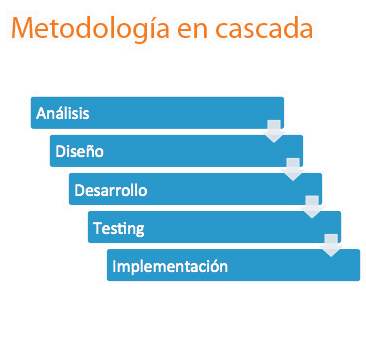
\includegraphics[width=0.6\textwidth]{imagenes/metodologia/meto_clasica.jpg}
    \caption{Etapas de la metodología clásica}
\end{figure}

\newpage

Dado que la metodología clásica sólo consta de un ciclo para realizar las etapas, será imprescindible una buena planificación de alcance, tiempo y coste del proyecto y de cada una de las etapas. Esta planificación inicial es tan importante porque no se obtendrán resultados del proyecto hasta que se encuentre cercano a su cierre.

Entre los problemas de la metodología clásica podemos encontrar los siguientes:

\begin{itemize}
    \item Los proyectos reales difícilmente se adecuan a este modelo de proceso.
    \item Dificultad para expresar por parte del cliente todos los requisitos al principio del proyecto.
    \item Poca comunicación con cliente/usuario, hasta las etapas finales no hay un ejecutable que se pueda evaluar.
\end{itemize}

\subsection*{Metodología Ágil}

La metodología ágil se caracteriza por una estructura incremental y un flujo de proceso iterativo. Esta metodología surge como solución a los problemas de la metodología clásica, sobretodo en la planificación de proyectos cortos y cambiantes. Esta metodología se adapta mejor a los proyectos del ámbito de las TIC, es decir, en el desarrollo de software. Esto es debido a que la metodología ágil consiste en la realización de continuas iteraciones, donde cada iteración da como resultado un prototipo del proyecto. Este modo de trabajar no se adecua a proyecto que puedan estar relacionados con el sector de la construcción, como puede ser la construcción de un puente, dado que no se pueden crear prototipos de una construcción ya que no serían seguros, y además son proyectos poco cambiantes en los requisitos del proyecto durante su desarrollo.

La metodología ágil está definida por las siguientes etapas:

\begin{figure}[h]
    \centering
    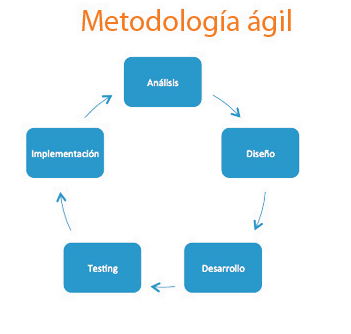
\includegraphics[width=0.6\textwidth]{imagenes/metodologia/meto_agil.jpg}
    \caption{Etapas de la metodología ágil}
\end{figure}

\section{Elección de la metodología}

La metodología que seguiré para el desarrollo de mi TFG es la metodología ágil. Pienso que es la metodología que más se adecua a las condiciones de mi proyecto, dado el limitado tiempo y la multitud de cambios que surgirán durante el desarrollo del mismo. Además la creación de prototipos ayudará a la mejora incremental de las funcionalidades del proyecto, teniendo en todo momento al menos un prototipo funcional que se pueda evaluar tanto por parte del tutor como del tribunal.

\chapter{Plataformas}

Un aspecto a tener en cuenta a la hora de elegir una plataforma para desarrollar un chatbot es que existen dos elementos en esta creación.

\begin{itemize}
    \item \textbf{Bot Frameworks}: son las plataformas encargadas de la creación y el alojamiento de los chatbots.
    \item \textbf{Bot Platforms}: son los entornos y aplicaciones donde van a ser desplegados los chatbots para su uso por parte de los usuarios.
\end{itemize}

A la hora de elegir la plataforma donde desarrollar el chatbot habrá que tener en cuenta que tanto el Bot Framework como el Bot Platform elegidos se adecuan a los requisitos del chatbot a crear.

Una posible clasificación de las plataformas puede ser en base al modo de creación de los chatbots. Dentro de esta clasificación encontramos las siguientes plataformas:

\begin{itemize}
    \item \textbf{Plataformas visuales}
    \item \textbf{Plataformas conversacionales}
    \item \textbf{Plataformas programables}
\end{itemize}

\subsubsection*{Plataformas visuales}

En estas plataformas no es necesario tener conocimientos técnicos para crear un chatbot. Por esta razón son las plataformas ideales para personas que no tienen conocimientos en programación ó IA. Algunos ejemplos de este tipo de plataformas pueden ser: Chatfuel y Octane AI. Esta simpleza en la creación del chatbot afecta en la posible complejidad que pueda tener el chatbot, por lo tanto no son las mejor opción para chatbots con con algo de complejidad, pero si para chatbots muy simples.

\subsubsection*{Plataformas conversacionales}

En estas plataforma es posible la creación de chatbots algo más complejos que en las plataformas visuales. Estos chatbots son capaces de mantener una conversación con un usuario, pero que a diferencia de los anteriores chatbots esta conversación no tiene un objetivo específico. Un posible ejemplo de este tipo de plataformas puede ser AIML, aunque AIML no es en sí una plataforma sino más bien un lenguaje de programación, si se convierte en una plataforma si se combina el lenguaje con alguna plataforma donde se permita al menos el alojamiento del chatbot. Este tipo de plataformas ya no está orientado a usuarios sin conocimientos técnicos, sino más bien a usuarios que tengan cierto nivel técnico y que busquen crear chatbots con cierta complejidad. 

\subsubsection*{Plataformas programables}

En estas plataforma se pueden crear desde los chatbots más simples hasta los más complejos. Para poder aumentar la complejidad se hace uso de técnicas de IA junto a las técnicas que ya se utilizaban en las anteriores plataformas, y aumenta la posibilidad de interactuar con servicios externos a la plataforma como pueden ser bases de datos y muchos más servicios. Algunos ejemplos de este tipo de plataformas pueden ser: Google Dialogflow, Microsoft Bot Framework y IBM Watson. \newline\newline


En la actualidad se dispone de un número elevado de plataformas capaces de crear chatbots de diferentes complejidades. De entre este número elevado de plataforma he seleccionado unas cuantas para analizarlas en detalle como posibles plataformas donde crear mi chatbot. En esta lista de plataformas no se encuentra ninguna plataforma visual dado que no posibilitan la complejidad necesaria para crear mi chatbot.


\section{AIML}

\subsection*{Información general}

El lenguaje de programación AIML (Artificial Intelligence Markup Language) fue desarrollado por el doctor Richard Wallace y la comunidad de código abierto Alicebot en la segunda mitad de los años 90. AIML es un lenguaje basado en etiquetas, al igual que los lenguajes HTML y XML. En concreto el lenguaje AIML se baso en gran medida en el lenguaje XML. Este parecido entre lenguajes no es una casualidad, si nos fijamos en el entorno de la época en la que se desarrollo AIML. A finales de la década de 1990 se produjo la explosión de la World Wide Web. Esta explosión trajo consigo al lenguaje HTML, que surgió como un lenguaje simple que sirviese como estándar para la creación de páginas web. El objetivo de HTML era que cualquier persona con pocos conocimientos informáticos fuese capaz de crear una página web. Esta filosofía de estándar de una tecnología y de simpleza la tomaron como ejemplo los creadores de AIML durante su desarrollo, intentando que AIML se convirtiese en un estándar en la creación de chatbots y que además fuese accesible al mayor número de usuarios. Además del lenguaje HTML, durante la década de 1990 se creo el lenguaje XML, que también se convirtió en un estándar.

Actualmente, al igual que le ha pasado al lenguaje HTML, el lenguaje AIML se ha ido actualizando con el tiempo añadiendo le nuevas funcionalidades que permitiesen crear chatbots más complejos, acorde al incremento de requisitos en los chatbots que ha ido surgiendo con el paso de los años. En el momento de la realización de este TFG, la última versión publicada de AIML es la versión 2.1 . Al crear agentes conversacionales con AIML, estos agentes no se convierten en cajas negras por lo tanto son más transparentes al programador que los creados con otras plataformas más grandes, ya que con AIML se crean chatbots basados en reglas. AIML se puede escribir en casi cualquier lenguaje natural.





→ http://www.aiml.foundation

\subsection*{Uso}

Para crear un chatbot con AIML es necesario generar una serie de archivos, que contendrán el estado y la configuración del bot.

En el estado del chatbot podemos distinguir el estado del bot y el estado del cliente. El estado del bot se define usando valores globales para las propiedades del bot, cada bot tendrá sus propiedades. El estado del cliente se define usando variables locales, cada cliente tendrá su estado específico.

La configuración del bot se define en los archivos AIML, en los archivos Learnf, en los Sets y en los Maps. Dentro de los archivos AIML se define la lógica del chatbot a base de añadir reglas, además en estos archivos se pueden realizar conexiones con otros chatbots definidos por otra serie de archivos. Dentro de los archivos Learnf se guardan las categorías aprendidas por el chatbot cuando en un template AIML se activa una etiqueta. Las categorías parendidas son globales a todos los clientes del chatbot. Dentro de los archivos Set se define un conjunto de cadenas. Dentro de los archivos Map se define un mapeo de cadena a cadena.

Según el estándar de AIML, esta serie de archivos se pueden definir dónde y cómo quiera el creador del chatbot.

Dado que AIML es sólo un lenguaje de programación, es necesario un framework para la creación del agente conversacional, como pueden ser algunos intérpretes y bibliotecas de código abierto (Python, Node JS, Java) ó servicios web (Pandorabots).

Si se elige la opción de usar intérpretes y bibliotecas de código abierto disponemos de las siguientes posibilidades:

\begin{itemize}
    \item Python $\rightarrow$ Program-Y
    \item Node JS $\rightarrow$ aimlinterpreter
    \item Java $\rightarrow$ Program AB
\end{itemize}

Si se elige la opción de usar servicios web como Pandorabots, uno de los más populares actualmente, se podrá alojar el chatbot en la plataforma y se podrá hacer uso de todas sus funcionalidades. Si nos centramos en Pandorabots disponemos de un editor de AIML, un editor de interfaces, control de versiones a través de Github, chatlogs, conversor de texto a voz y viceversa, posiblidad de añadir un personaje 3D como interación con el chatbot, integración con RESTful APIs y muchos más, según se indica en su página oficial (referencia a https://developer.pandorabots.com/).

Muchas de estas funcionalidades depende del tipo de cuenta que se disponga en Pandorabots.

\newpage

\begin{figure}[h]
    \centering
    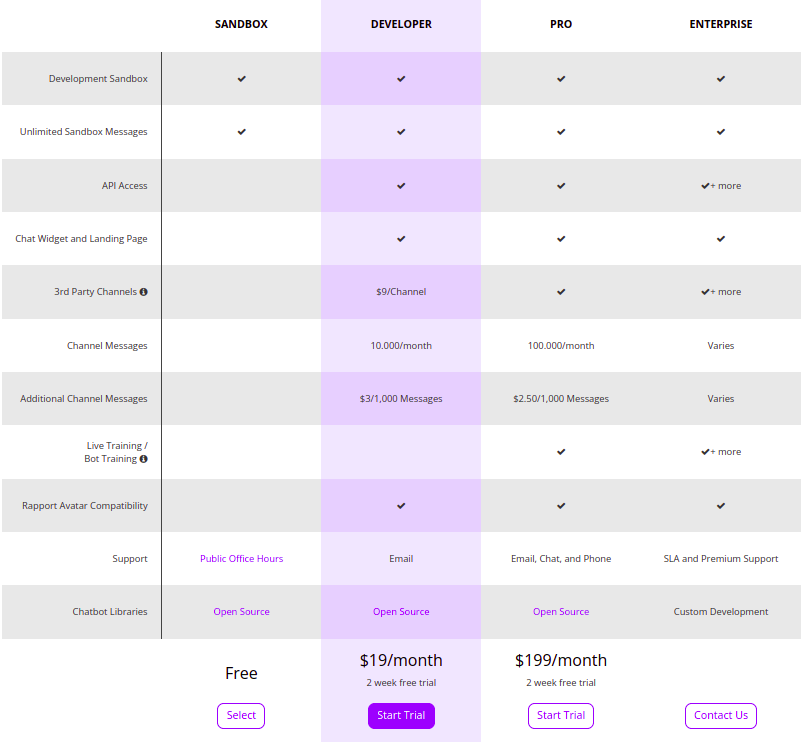
\includegraphics[width=1.0\textwidth]{imagenes/plataformas/cuentas_pandorabots.png}
    \caption{Cuentas disponibles en Pandorabots (Fuente: developer.pandorabots.com)}
    \label{fig:cuenta_pandorabots}
\end{figure}

En la figura \ref{fig:cuenta_pandorabots} podemos comprobar como con la cuenta gratuita no disponemos de todas las funcionalidad anteriormente descritas.


→ https://developer.pandorabots.com/


\subsection*{Extensibilidad}

Dado que hay muchos frameworks para la creación de un chatbot con AIML, dependerá del framework elegido la cantidad de posiblidades de conexiones con APIs o servicios externos al chatbot. 

Para que AIML sea flexible y extensible dispone de la posibilidad de integrar sus propias API's, bases de datos ó también se pueden crear etiquetas propias; pero para ello se debe tener cierto nivel con el lenguaje de programación AIML.

Si optamos por servicios web como Pandorabots para poder disponer de conexión con servicios externos al servicio web o con APIs se debe disponer de una cuenta de pago, no basta con la versión gratuita de Pandorabots.

\subsection*{Integración}

Si optamos por servicios web como Pandorabots, al igual que pasa con la extensibilidad, será necesaria una cuenta de pago para poder integrar nuestro chatbot en plataformas de mensajería como Facebook Messenger, Twitter, Telegram y muchos más.

Pero si optamos por framework de código abierto hay una multitud de posibilidades, tantas como nivel de conocimientos tenga el creador del chatbot. Un ejemplo puede ser con Node JS, donde podríamos desplegar el chatbot en cualquier página web a través de una interfaz web que enviase peticiones al servidor creado con Node JS que aloja al chatbot.


\section{IBM Watson}

\subsection*{Información general}

IBM Watson es un portfolio de IBM de aplicaciones, herramientas y soluciones preparadas para la empresa, diseñado para reducir los costes y los obstáculos de IA, además de optimizar los resultados y el uso responsable de la IA según se indica en su página oficial (referencia a https://www.ibm.com/es-es/watson). Aunque en un inicio IBM Watson no era lo que es ahora actualmente y tampoco se buscaba llegar a este punto. Originalmente IBM Watson surgío como el siguiente gran desafío de la empresa IBM, tras haber salido victorioso de otros grandes desafíos como la victoria de Deep Blue contra Garry Kasparov y el desafío de la supercomputadora Blue Gene. El objetivo que perseguía en sus orígenes Watson era conseguir ganar a competidores humanos en el concurso Jeopardy. Este concurso de televisión estadounidense consistía en un concurso de preguntas sobro una multitud de temas, y los concursantes deberán resolver las preguntas de cada prueba realizando preguntas sobre las pistas que va dando el presentador. Las reglas del concurso obligan a que Watson no sólo sepa conocimientos sobre los temas que se utilizan en el concurso, sino también ha saber realizar preguntas al presentador en base a sus pistas, y además saber distinguir cuando la pista del presentador no es cierta. Todas estos requisitos convierten el ganar este concurso en un gran desafío, la empresa IBM se embarco en este proyecto a mediados de la década del 2000. Finalmente en el año 2011 se llegó a un acuerdo para la realización del programa, donde compitieron dos grandes exconcursantes del programa como son Ken Jennings y Brad Rutter contra Watson. Tal y como se indica en el articulo (referecia a https://www.techrepublic.com/article/ibm-watson-the-inside-story-of-how-the-jeopardy-winning-supercomputer-was-born-and-what-it-wants-to-do-next/), Watson ganó el juego con \$77,147 , dejando a Rutter y Jennings con \$21,600 y \$24,000 respectivamente.

Tras la victoria de IBM Watson, se empezó a enfocar y rediseñar a Watson hacia distintos sectores como la medicina, la banca ó los agentes conversacionales entre otras. Los agentes conversacionales es el sector que nos interesa investigar.

Dado que IBM Watson está orientado al mundo empresarial destaca por su confianza, es decir, Watson es transparente en cuanto a las decisiones basadas en IA; también protege la privacidad de los datos y su seguridad. Todas estas características son muy valoradas en cualquier producto empresarial, incluso algunas son imprescindibles.

Otro característica de Watson es su procesamiento del lenguaje natural. Al igual que AIML es multilenguaje, pero Watson lo lleva a un aspecto más complejo añadiendo la capacidad de analizar datos complejos y no estructurados, como pueden ser códigos de programación ó incluso formas de expresión específicas de una modalidad de trabajo. Este procesamiento del lenguaje natural no es algo alcanzable por cualquier empresa. La IA de Watson sabe desenvolverse en la situaciones más complejas, como pueden ser situaciones en las que no pueda responder, reenviando la solicitud a un agente humano o hacia algún documento de ayuda; evitando realizar preguntas redundante facilitando la comunicación y haciéndola más natural; y por última sabe manejar solicitudes ambiguas comunes en la comunicación como pueden ser errores ortográficos, cambios de tema, y muchas más situaciones que pueden ser inesperadas para el chatbot en una conversación. Además IBM Watson intenta mejorar su rendimiento aportando al creador del chatbot información sobre que nuevos temas añadir para mejorar la respuesta a las solicitudes.

Y por último destaca que Watson trabaja con cualquier servicio en la nube, lo que facilita su integración en las empresas, ya que no será un impedimento el lugar donde residan los datos de la empresa. Y además el trabajar en cloud facilitará el trabajo con los datos.

En concreto en la página oficial de IBM Watson Assistant (referencia a https://www.ibm.com/es-es/products/watson-assistant) se destaca la rentabilidad del producto, de hasta un 337\% según el Informe TEI de Forrester (referencia a El Total Economic Impact™ de IBM Watson Assistant); su precisión, de hasta un 14,7\% superior que las soluciones de la competencia según un reciente estudio publicado sobre machine learning (referencia a https://www.ibm.com/blogs/watson/2020/12/watson-assistant-improves-intent-detection-accuracy-leads-against-ai-vendors-cited-in-published-study/); y su fiabilidad, ya que Watson tiene más de 1000 despliegues de clientes en todos los sectores.



→ https://www.ibm.com/es-es/watson

→ El Total Economic Impact™ de IBM Watson Assistant

→ https://www.ibm.com/es-es/products/watson-assistant

→ https://www.techrepublic.com/article/ibm-watson-the-inside-story-of-how-the-jeopardy-winning-supercomputer-was-born-and-what-it-wants-to-do-next/

→ https://www.ibm.com/blogs/watson/2020/12/watson-assistant-improves-intent-detection-accuracy-leads-against-ai-vendors-cited-in-published-study/

\subsection*{Uso}

IBM Watson está pensado para ser utilizado por cualquier persona, da igual que no tenga conocimientos en programación. La creación del chatbot se basa en un editor de arrastrar y soltar. Este editor evita la complejidad de la programación de un chatbot y los posibles errores derivados de esa necesidad de escribir el código en su creación ó en alguna modificación que necesite el chatbot. Es posible crear un chatbot sin escribir una sola línea de código.

\begin{figure}[h]
    \centering
    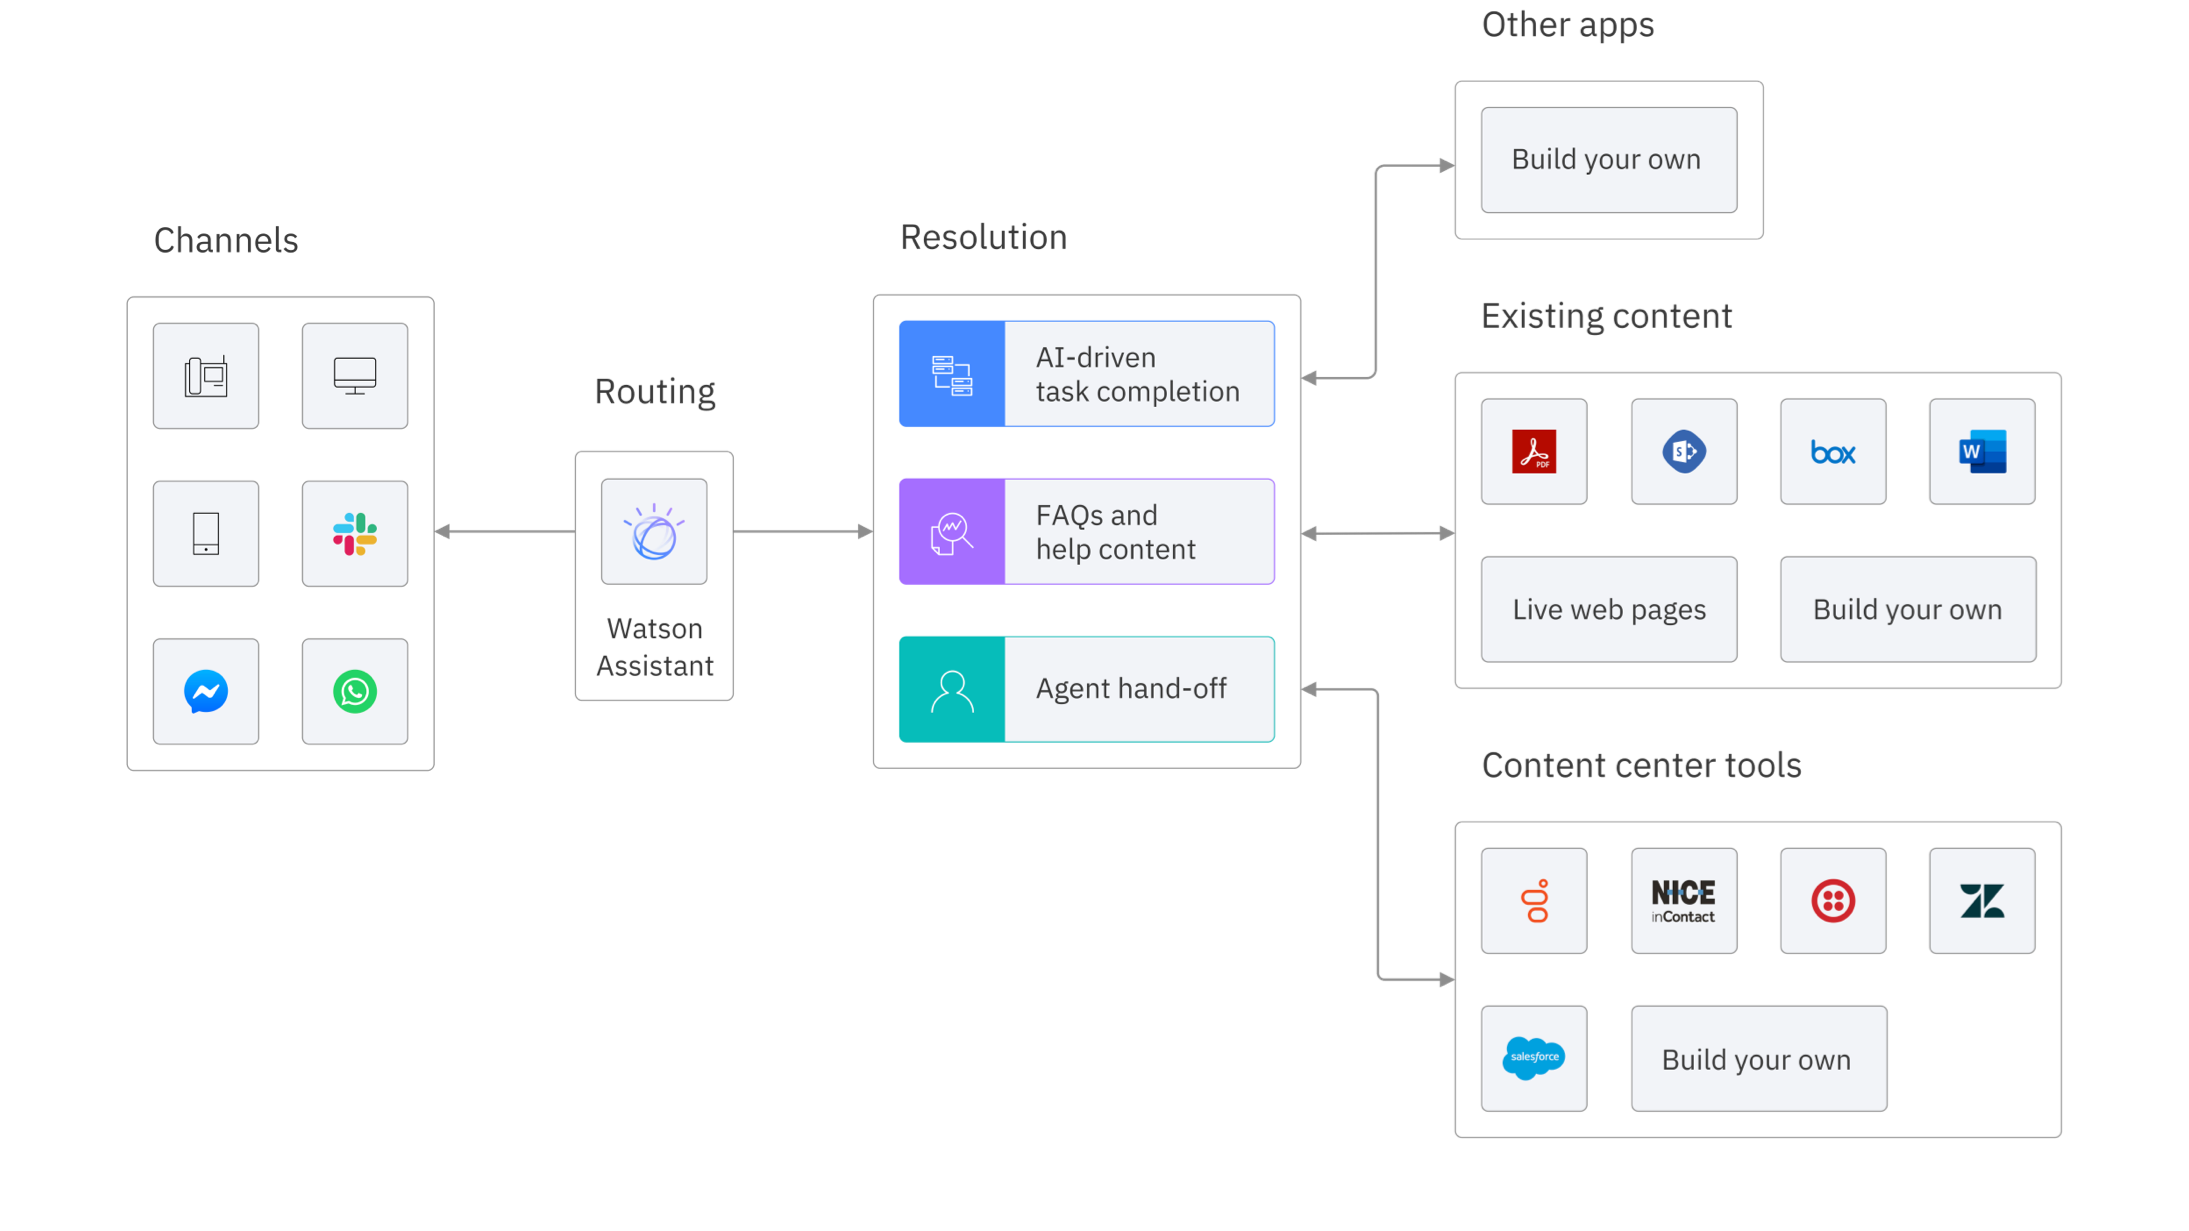
\includegraphics[width=1.0\textwidth]{imagenes/plataformas/editor_IBM_Watson.png}
    \caption{Editor de IBM Watson (Fuente: ibm.com/es-es/products/watson-assistant)}
\end{figure}

La IA del chatbot es capaz de comprender un tema en cualquier lenguaje natural con unas pocas frases facilitando la adaptación del chatbot a la funcionalidad que se le quiera dar, adaptándose de forma rápida y precisa al dominio del proyecto.

\subsection*{Extensibilidad}

Como se ha indicado en apartados anteriores, IBM Watson es un portfolio de IBM de aplicaciones. En su página oficial (referencia a https://www.ibm.com/es-es/watson/products-services) se indican las siguientes aplicaciones con las que se puede integrar el chatbot:

\begin{itemize}
    \item IBM Watson Discovery
    \item IBM Watson Natural Language Understanding
    \item IBM Watson Speech to Text
    \item IBM Watson Text to Speech
    \item IBM Watson Knowledge Studio
    \item IBM Watson Language Translator
    \item IBM Watson Natural Language Classifier
\end{itemize}

Entre estas aplicaciones se encuentran algunas muy útiles como IBM Watson Discovery para la extracción y búsqueda de información, IBM Watson Speech to Text para transformar la voz a texto escrito gracias a una potente tecnología de machine learning, IBM Watson Language Translator para traducir dinámicamente información, ó IBM Watson Knowledge Studio para enseñar a Watson el idioma del domino del chatbot.



→ https://www.ibm.com/es-es/watson/products-services

\subsection*{Integración}

El chatbot se puede integrar como un chat web, como contestador de llamadas de teléfono ó como un chatbot en una aplicación de mensajería como WhatsApp, Facebook Messenger, SMS y muchos más. Todas estas formas de integrar el chatbot son muy fáciles de realizar.


\section{Google Dialogflow}

\subsection*{Información general}

Dialogflow pertenece a la empresa Google, aunque no fue desarrollada originalmente por ella. Google adquirío API.AI en el año 2016 y le cambió el nombre a Dialogflow. Desde su adquisición Google a mejorado Dialogflow gracias a sus técnicas de IA de gran calidad. Esta plataforma es una de las más utilizadas para la creación de chatbots junto con IBM Watson, aunque a diferencia de Watson, Dialogflow está enfocado tanto para el mundo empresarial como para usuarios particulares que están empezando en el mundo de los chatbots. Esta variedad en la complejidad del chatbot es posible gracias a una interfaz que permite crear un chatbot con unos mínimos conocimientos técnicos, sólo será necesario introducir las frases de las preguntas y de las respuestas para construir el chatbot. Y si se quiere crear un chatbot más complejo podemos introducirnos en la configuración del chatbot o integrar más funcionalidades que aumenten su complejidad.

Dentro de Dialogflow existen dos tipos de agentes, los Agentes de ES y los agentes de CX. Dentro de los agentes de ES existen dos ediciones, la edición de prueba y la edición Essentials. Con la versión de prueba no se puede acceder a los servicios de Google Cloud, pero las entradas y salidas son gratuitas; mientras que con la versión Essentials si se puede acceder a esos servicios, pero las entrada y salidas del agente empezarán a costar dinero. Entre la versión Essentials y la versión CX la principal diferencia es que en la versión CX la relación entre los intents se define mediante un diagrama de flujo, mientras que en la versión Essential la relación entre los intents se define mediante los contextos. La limitación de los contextos es que no posibilitan la relación de varios intents con otro intent. La versión CX ha sido lanzada hace pocos unos pocos meses por lo que es algo novedosa y es útil para aquellos que quieran realizar un chatbot algo más complejo o que ya tengan experiencia con la plataforma. La versión Essentials está más enfocada a agentes de complejidad media y la versión CX está más enfocada a agentes de complejidad alta.

\subsection*{Uso}

Para empezar a crear un chatbot con Dialogflow será necesaria una cuenta Google. Los apartados claves para la creación de un bot son Intents y Entities.

Dentro del apartado Intents se crean los distintos intents a usar en el chatbot, cada intent es un estado al que accede el chatbot si se cumple el contexto y se detecta una de las frases de entrenamiento del intent. Los contextos sirven para guardar información adquirida que puede resultar útil durante la conversación, como el nombre del usuario que está usando el chatbot; además de la información que se quiere conservar también se puede indicar durante cuento tiempo se estima que es útil esa información, también llamado lifespan. Dentro de cada intent se debe también definir las posibles respuestas que envía el chatbot si se activa el intent. Y por último a cada intent se le pueden añadir eventos. Por defecto en el apartado Intents vienen creados los siguientes intents:

\begin{itemize}
    \item Default Fallback Intent: Intent para cuándo el chatbot no reconoce la pregunta
    \item Default Welcome Intent: Intent para dar la bienvenida al chatbot
\end{itemize}

Dentro del apartado Entities se crean las distintas entidades. Una entidad es un conjunto de ejemplos sobre un tema, por ejemplo la entiedad paises contiene los siguientes elementos: España, Francia, Italia, etc. Cuando se define una entidad se deben indicar los elementos que la forman, pero adicionalmente se puede indicar los sinónimos de los elementos, este añadido le dará una mayor naturalidad a la conversación al hacer que los textos no sean tan estáticos.

Otro apartado importante para el desarrollo del chatbot es el apartado Training, donde se podrán analizar las conversaciones que se han realizado con el chatbot e indicar si se ha respondido adecuadamente o no, esta acción de aceptación o no hará que el chatbot sea más preciso con sus respuestas. Si se acepta una respuesta, si la pregunta realizada por el usuario no se encuentra entre las preguntas del intent activado, se añade a la lista de preguntas del intent.

\subsection*{Extensibilidad}

Dialogflow permite integrar un webhook. Este webhook puede estar alojado tanto en un servidor externo como en Google Cloud. Si se opta por la opción de Google Cloud, para lo que es necesario una cuenta Google de pago, se pueden añadir los archivos que componen el webhook en el apartado Fulfillment dentro de un editor en linea. Si se opta por la opción de un servidor externo, tanto si es local como si es en una plataforma en la nuebe, se deberá añadir la URL del servidor web en el mismo apartado que se indicó anteriormente. La conexión con el servidor externo se realizará mediante el envío de peticiones tipo POST. Estas peticiones contendrán la información en formato JSON. Para que la información se envíe al servidor, independientemente de la opción que se elija, se debe activar en los intents elegidos la opción del webhook, de esta forma cuando se active el intent se enviará una petición al servidor web.

Una vez se tenga una conexión con un servidor web, dentro de este servidor se podrán añadir más funcionalidad, como BBDD ó interpretes de AIML, que permitirán seguir extendiendo el chatbot.

\subsection*{Integración}

El chatbot se puede integrar en canales de telefonía, como Twilio; en canales de mensajería, como Telegram, Facebook Messenger ó Twitter; en canales de videollamadas, como Skype; y en páginas web en forma de chat web.


\section{Rasa Stack}

\subsection*{Información general}

Rasa Stack es un conjunto de herramientas de aprendizaje automático de código abierto para el desarrollo de chatbots. Rasa Stack está desarrollado por una comunidad de personas pertenecientes a muchos lugares del mundo, de modo que esta plataforma a diferencia de las dos anteriores, no está respaldado por ninguna de las grandes empresas tecnológicas como pueden ser Google o IBM. Pero esto no quiere decir que no sea una buena plataforma, ya que ha sido probada por grandes empresas como AIRBUS, TOYOTA ó Adobe.

En su página oficial (referencia a https://rasa.com) se destaca la gran personalización que pueden alcanzar los chatbots en esta plataforma.

Dentro de Rasa Stack se pueden distinguir dos tipos de cuenta, la cuenta para empresas (Rasa Enterprise) y la cuenta gratuita (Rasa Open Source ó Rasa X). La diferencia entre Rasa Open Source y Rasa X es que Rasa X no es de código abierto, mientras que Rasa Open Source, como indica su nombre, si es de código abierto. La cuenta para empresas proporciona funcionalidades muy útiles para productos empresariales como pueden ser realizar análisis del chatbot, acceso con roles a la plataforma, disponibilidad de un soporte de calidad, y mucho más.

En Rasa Stack se destaca que los chatbot creados en esta plataforma no se convierten en cajas negras, sino que el funcionamiento del chatbot es transparente, por lo tanto se tiene total acceso a la configuración de todo el chatbot, incluido el modelo usado en el entrenamiento del bot.


→ https://rasa.com

\subsection*{Uso}

Al igual que pasa en Dialogflow, Rasa Stack mantiene un contexto de la conversación, donde se guarda información proporcionada por el usuario, lo que permite una conversación más natural al no realizar preguntas redundantes.

La creación del chatbot se divide en dos módulos, Rasa NLU y Rasa Core. La plataforma proporciona un NLU avanzado, Rasa NLU, esta NLU se puede entrenar en base a una lista de mensajes, a cada mensaje se le asignará una intención y las entidades que contiene. Una vez está entrenado el módulo NLU, se procede a configurar el módulo Rasa Core, que es el encargado de confeccionar la respuesta del chatbot a la pregunta identificada por el módulo Rasa NLU. La configuración de Rasa Core consiste en escribir las respuestas de los distintos intents, definir el dominio del chatbot, definir la conexiones con APIs, y definir el modelo de gestión del diálogo, por ejemplo una CNN, citando además las políticas que se van a usar.

\subsection*{Extensibilidad}

La transparencia que tienen los chatbots permiten conectar con él muchas APIs externas que suman más funcionalidades a parte de las que ya proporciona la plataforma. Y al igual que pasa con Dialogflow, se puede conectar a un servidor web y al servidor las APIs.

\subsection*{Integración}

Tal y como se indica en su página oficial (referencia a https://rasa.com), un chatbot creado con Rasa Stack se puede integrar en canales como IVR, chat y SMS. Además se indica que Rasa Stack admite 10 canales de mensajería integrados, como pueden ser Telegram, Facebook Messenger, Slack y algunos más; y que adicionalmente proporciona un punto de conexión con cualquier plataforma de comunicación, como puede ser un servidor web.


\section{Comparativa}


\begin{table}[h]
\centering
\resizebox{\textwidth}{!}{%
\begin{tabular}{|c|l|l|}
\hline
\multicolumn{1}{|l|}{} &
  \multicolumn{1}{c|}{\textbf{PROS}} &
  \multicolumn{1}{c|}{\textbf{CONTRAS}} \\ \hline
\textbf{AIML} &
  \begin{tabular}[c]{@{}l@{}}- Multilenguaje\\ - El chatbot no es un caja negra\\ - Lenguaje de programación simple\\ - Posibilidad de conexión con APIs propias\\ - Muchas funcionalidades de forma gratuita\end{tabular} &
  \begin{tabular}[c]{@{}l@{}}- Alto gasto de tiempo en la creación del agente conversacional\\ - Necesidad de una cuenta de pago usando servicios web\\ - No es una plataforma en la nube\end{tabular} \\ \hline
\textbf{IBM Watson} &
  \begin{tabular}[c]{@{}l@{}}- Posibilidad de crear chatbots muy complejos\\ - Gran cantidad de conexiones con APIs de mucha calidad\\ - Editor de arratrar y soltar\\ - Facilidad de desplegar el chatbot en muchos canales importantes\\ - Es una plataforma en la nube\end{tabular} &
  \begin{tabular}[c]{@{}l@{}}- Necesidad de una cuenta de pago para crear chatbot complejos\\ - Enfocado para el mundo empresarial\\ - El chatbot es una caja negra\end{tabular} \\ \hline
\textbf{Dialogflow} &
  \begin{tabular}[c]{@{}l@{}}- Posibilidad de crear chatbots muy complejos sin necesidad de pago\\ - Posibilidad de conexión con un servidor web de forma gratuita\\ - Facilidad de desplegar el chatbot en muchos canales importantes\\ - Creación de chatbots usando sólo frases y entidades\\ - Es una plataforma en la nube\end{tabular} &
  \begin{tabular}[c]{@{}l@{}}- Para hacer agentes muy complejos es necesario gastar tiempo en la creación del servidor\\ - Se necesita tener cierto conocimiento de la plataforma para sacar todo su potencial\\ - Calidad regular en la documentación\\ - Parte del chatbot es una caja negra\end{tabular} \\ \hline
\textbf{Rasa Stack} &
  \begin{tabular}[c]{@{}l@{}}- Documentación de calidad\\ - El chatbot no es un caja negra\\ - Facilidad de desplegar el chatbot en muchos canales importantes\\ - Posibilidad de crear chatbots muy complejos\end{tabular} &
  \begin{tabular}[c]{@{}l@{}}- Necesidad de alto nivel técnico\\ - Plataforma en desarrollo\\ - Necesidad de mucho tiempo para la creación del chatbot\\ - No es una plataforma en la nube\end{tabular} \\ \hline
\end{tabular}%
}
\caption{Comparativa de las plataformas de desarrollo}
\label{tab:my-table}
\end{table}


%\input{capitulos/01_Introduccion}
%
%\input{capitulos/02_EspecificacionRequisitos}
%
%\input{capitulos/03_Planificacion}
%
%\input{capitulos/04_Analisis}
%
%\input{capitulos/05_Diseno}
%
%\input{capitulos/06_Implementacion}
%
%\input{capitulos/07_Pruebas}
%
%\input{capitulos/08_Conclusiones}
%
%%\chapter{Conclusiones y Trabajos Futuros}
%
%
%%\nocite{*}
\bibliographystyle{plainnat}
\bibliography{bibliografia/bibliografia}\addcontentsline{toc}{chapter}{Bibliografía}
%
%\appendix
%\input{apendices/manual_usuario/manual_usuario}
%%\input{apendices/paper/paper}
%\input{glosario/entradas_glosario}
% \addcontentsline{toc}{chapter}{Glosario}
% \printglossary
\chapter*{}
\thispagestyle{empty}

\end{document}
